% Diapositiva 20
% Kevin
%=============================================
% 1. Explicar qué significa comparar amplitudes observadas y predichas.
%=============================================

\begin{frame}{Comparación de Amplitudes: Lógica Inversa}

    \begin{columns}[T]
        %========================================
        % COLUMNA IZQUIERDA: VISUALIZACIÓN
        %========================================
        \column{0.52\textwidth}
        \begin{center}
            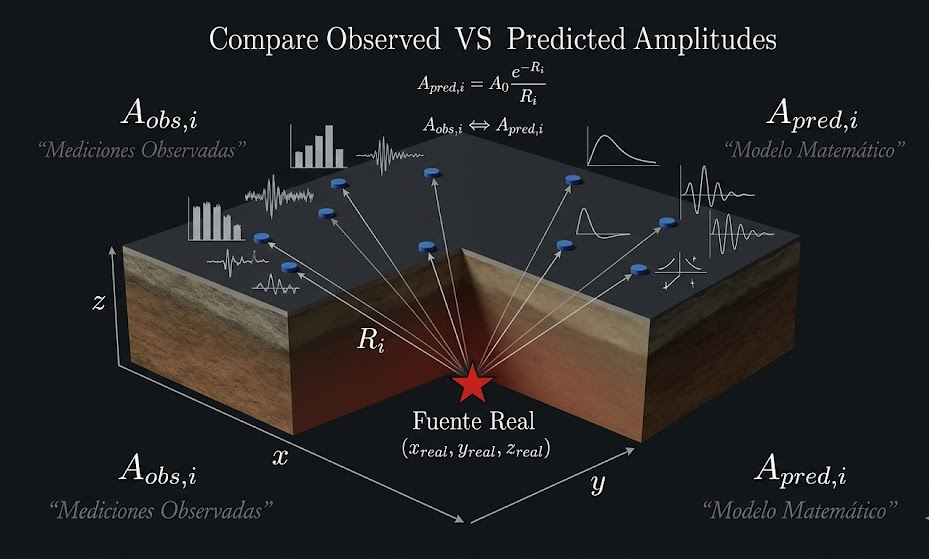
\includegraphics[width=0.95\textwidth]{Imagenes/AmplitudesObservadasPredichas.png}
        \end{center}

        \vspace{-0.2cm}
        \begin{center}
            \tiny \textcolor{gray}{
            Contraste entre mediciones ruidosas y el modelo teórico.
            }
        \end{center}

        %========================================
        % COLUMNA DERECHA: FUNDAMENTO TÉCNICO
        %========================================
        \column{0.44\textwidth}
        
        \begin{block}{Fundamento Inverso}
            \scriptsize 
            \begin{itemize}
                \item \textbf{Diferencial:} Contraste entre registradas ($A_{obs}$) y teóricas ($A_{pred}$).
                \vspace{0.2cm}
                \item \textbf{Criterio:} El ajuste óptimo indica proximidad a la fuente real.
                \vspace{0.2cm}
                \item \textbf{Convergencia:} 
                \[ A_{pred} \approx A_{obs} \implies \text{Proximidad} \]
            \end{itemize}
        \end{block}

        \begin{exampleblock}{Modelo Matemático}
            \centering
            \footnotesize
            \[ A_{pred,i} = A_0 \frac{e^{-R_i}}{R_i} \]
        \end{exampleblock}

    \end{columns}

    \vspace{0.3cm} 
    \begin{center}
        \footnotesize 
        \textbf{Minimizar la discrepancia entre la física y la medición.}
    \end{center}

\end{frame}